\documentclass[11pt,a4paper,twoside,pdf]{article}

% Paquetes (añade otros si los necesitas):
\usepackage{latexsym}
\usepackage[utf8x]{inputenc}
\usepackage{soul}
\usepackage{array}
\usepackage{amsmath}
\usepackage{amssymb}
\usepackage{marvosym}
\usepackage{epsfig}
\usepackage{graphics}
\usepackage{amsfonts}
\usepackage{xspace}
\usepackage{color}
\usepackage{booktabs}
\usepackage{xtab}
\usepackage[colorlinks=true,urlcolor=blue,linkcolor=blue,citecolor=blue]{hyperref}
\numberwithin{equation}{section}

% Fuente: palatino
\usepackage[sc]{mathpazo}
\linespread{1.05}

% TFG en inglés:
%\usepackage[english]{babel} 
%\addto\captionsenglish{\renewcommand{\chaptername}{}}

% TFG en español:
\usepackage[spanish,es-nodecimaldot,es-tabla,es-lcroman,es-nosectiondot,
            es-noindentfirst]{babel}
\renewcommand\spanishchaptername{}

% Formato de la página:
\usepackage{fancyhdr}
\usepackage[top=2.88cm,bottom=2.97cm,left=2.95cm,right=2.95cm]{geometry}
\setlength{\parskip}{0.1cm}

% Pon aquí tus definiciones:

\newcommand{\dis}{\displaystyle}
\sodef\an{}{.2em}{1em plus1em}{2em plus.1em minus.1em}

\begin{document}

% Portada %%%%%%%%%%%%%%%%%%%%%%%%%%%%%%%%%%%%%%%%%%%%%%%%%%%%%%%%%%%%%%%%%%%%%%

\pagestyle{empty}


\noindent
\begin{tabular}{r}

\includegraphics[width=8.8cm]{escudoUGRmonocromo.png} \\[-1.8ex]
\hspace{31mm}\vspace{-8mm}
\begin{tabular}{c}
\hline\\[-1ex]\hskip-2mm
{\bf Facultad de Ciencias}\hspace{18mm}
\end{tabular}
\end{tabular}

{\large
\vspace{30mm}
\hspace{25mm}
\begin{tabular}{l}
\an{GRADO EN FISICA}
\end{tabular}

\vspace{45mm}
\hspace{25mm}
\begin{tabular}{l}
\an{TRABAJO FIN DE GRADO}
\\[1.5ex]
\an{\LARGE\bf IMPLEMENTACI\'ON DE }
\\
\an{\LARGE\bf M\'ETODOS}
\\
\an{\LARGE\bf EN DIFERENCIAS FINITAS }
\\
\an{\LARGE\bf EN GPUs}
\end{tabular}

\vfill
\hspace{25mm}
\begin{tabular}{l}
Presentado por:
\\
{\bf D. JUAN JOS\'E SALAZAR L\'OPEZ}
\\[3ex]
Curso Académico 2021/2022
\end{tabular}
}


\newpage

\begin{center}

{\bf Resumen}
\bigskip

\begin{minipage}{0.8\linewidth}
En el siguiente TFG se procede a presentar las ventajas de aplicar el método de diferencias finitas en el dominio del tiempo (FDTD) en GPU, a diferencia del modo de aplicación usual el cual se lleva a cabo usando la potencia de cálculo de las CPUs. La principal diferencia radica en el poder de paralelización de las GPUs, el cual nos proporciona al implementar el método en $\mathbb R^{2}$ una disminución en el tiempo de cálculo de las ecuaciones de Maxwell de aproximadamente un orden de magnitud.

%\El método numérico de las diferencias finitas en el dominio del tiempo (FDTD) se usa como herramienta para %\la resolución de ecuaciones diferenciales de primer orden.  Este cobra especial importancia en la %\electrodinámica computacional dado que nos permite resolver las ecuaciones de Maxwell realizandoalgoritmos %\con los que calcular punto a punto los valores del campo electromagnético. Estos algoritmos se implementan %\generalmente usando la potencia de cálculo que nos proporcionan las CPUs y dada la necesidad dediscretizar %\el espacio, el timepo empleado en el proceso de cálculo aumenta con las dimensiones del problema. En este %\TFG se han generado varios algoritmos de uso libre en CUDA para exponer las ventajas que se obtienen al %\implementar este método usando el poder de paralelización que nos proporcionan las GPUs, lo que disminuyeel %\tiempo empleado en el cálculo de los campos. 
\end{minipage}

\vfill

{\bf Abstract} 
\bigskip

\begin{minipage}{0.8\linewidth}
In the following TFG it is shown the advantages of implementing the finite difference time domain method (FDTD) in GPU, instead of using the calculus power of CPUs. The principal difference is the parallelization power of the GPUs which allows us to decrease the calculus time to solve the Maxwell equations in about one order of magnitude when we implement the method in $\mathbb R^{2}$.
\end{minipage}

\vfill

\end{center}

% Indice %%%%%%%%%%%%%%%%%%%%%%%%%%%%%%%%%%%%%%%%%%%%%%%%%%%%%%%%%%%%%%%%%%%%%%%
\newpage

\tableofcontents

% Texto %%%%%%%%%%%%%%%%%%%%%%%%%%%%%%%%%%%%%%%%%%%%%%%%%%%%%%%%%%%%%%%%%%%%%%%%
\newpage

\pagestyle{fancy}
\fancyhead[RO,LE]{\leftmark}
\fancyhead[LO,RE]{\thepage}
\fancyfoot{}

\section{Introducción}
El método numérico de las diferencias finitas es usado en muchos campos para la resolución de ecuaciones diferenciales de primer orden \cite{Taflove2005}. En particular, el método de la diferencia central finita cobra especial importancia en la electrodinámica computacional donde se emplea para resolver las ecuaciones de Maxwell en el dominio del tiempo, discretizando tiempo y espacio para poder implementar la solución en un algoritmo.
Actualmente su uso está muy extendido ya que posibilita el estudio de la propagación de señales electromagnéticas por diversos medios. En particular puede usarse para determinar la radiación que actúa sobre una cabeza humana producida por un teléfono móvil o la propagación de una señal en el uso de radares marítimos entre otras aplicaciones.

Desde que se desarrolló el método y se generaron los primero algoritmos se ha hecho uso del poder de cómputo que nos proporcionan las CPUs, el cual ha ido creciendo con el paso de los años. No obstante, al aumentar el tamaño del modelo también aumenta el tiempo necesario para obtener la solución dado que se debe calcular punto a punto los valores de los campos al aplicar el método. Este problema puede solventarse haciendo uso del poder de paralelización que nos ofrecen las tarjetas gráficas (GPUs), pudiendo hacer simultaneamente, hasta cierto límite, todas las operaciones necesarias en cada coordenada de la dimensión espacial. Proceso que se consigue implementando los algoritmos FDTD en el lenguaje CUDA, con el cual podemos podemos determinar un conjunto de hilos para realizar los cálculos simultaneamente.


\url{https://github.com/juanjo1213/TFG-FDTD}



\section{Metodología}
\subsection{El método de diferencias finitas en el dominio del tiempo}
El método numérico de las diferencias finitas se emplea en la resolución de ecuaciones diferenciales de primer orden, en particular, el método de la diferencia central finita se basa en aproximar de forma sencilla la derivada de una función en un punto como la diferencia de dicha función evaluada en dos puntos equidistantes al mismo. Haciendo uso del desarrollo en serie de Taylor y aproximando a segundo orden obtenemos:

\begin{equation}
f(x+h)=y(x)+hy^\prime(x)+\frac{h^3}{2}y^{\prime\prime}(x)+\frac{h^3}{6}y^{\prime\prime\prime}(x)
\end{equation}

\begin{equation}
f(x-h)=y(x)-hy^\prime(x)+\frac{h^3}{2}y^{\prime\prime}(x)-\frac{h^3}{6}y^{\prime\prime\prime}(x)
\end{equation}

\begin{equation}
y\prime(x)=\frac{y(x+h)-y(x-h)}{2h}+O(h^2)
\end{equation}

Donde hemos despejado el valor de la derivada de la función en un punto mediante su desarrollo en serie en $(x+h)$ y $(x-h)$.

Recordando la expresión de las ecuaciones de Maxwell para el campo electromagnético, haciendo uso del vector campo $D$.

\begin{equation}
\frac{\partial D}{\partial t}=\nabla \times H
\end{equation}

\begin{equation}
\frac{\partial H}{\partial t}=-\frac{1}{\mu_{0}}\nabla \times E
\end{equation}

\begin{equation}
D(\omega)=\varepsilon_{0}\varepsilon^*_{r}(\omega)E(\omega)
\end{equation}

Podemos observar que están expresadas en el dominio de la frecuencia para poder aplicarlas a medios cuya constante dieléctrica dependa de la misma. Resaltar que $\varepsilon_{0}$ y $\varepsilon_{r}$ corresponden con las constantes dieléctricas del vacío y del medio respectivamente, y $\mu_{0}$ es la permeabilidad magnética del vacío.


Para simplificar el formalismo es conveniente normalizar las ecuaciones haciendo uso de las constantes dieléctrica y permeabilidad magnética del vacío.
\begin{equation}
\tilde{E}=\sqrt{\frac{\varepsilon_{0}}{\mu_{0}}}E
\end{equation}

\begin{equation}
\tilde{D}=\frac{1}{\sqrt{\varepsilon_{0}\mu_{0}}}D
\end{equation}

De este modo podemos expresar las ecuaciones de Maxwell para el campo electromagnético como:

\begin{equation}
\frac{\partial \tilde{D}}{\partial t}=-\frac{1}{\sqrt{\varepsilon_{0}\mu_{0}}}\nabla \times H
\end{equation}

\begin{equation}
\frac{\partial H}{\partial t}=-\frac{1}{\sqrt{\varepsilon_{0}\mu_{0}}}\nabla \times E
\end{equation}

\begin{equation}
\tilde{D}(\omega)=\varepsilon^*_{r}(\omega)\tilde{E}(\omega)
\end{equation}


En $\mathbb R^{3}$ tenemos 3 componentes para el campo eléctrico y 3 para el magnético $\tilde{E}_{x}$, $\tilde{E}_{y}$, $\tilde{E}_{z}$, $H_{x}$, $H_{y}$, $H_{z}$, por lo que, si queremos aplicar un modelo en dos dimensiones debemos elegir uno de los dos grupos de tres vectores, (i) el transversal magnético, formado por $\tilde{E}_{z}$, $H_{x}$, $H_{y}$, o (ii) el transversal eléctrico, compuesto por los vectores $\tilde{E}_{x}$, $\tilde{E}_{y}$ y $H_{z}$.

Usaremos el modo transversal magnético y utilizaremos directamente las letras E y D sin tildar para nombrar a las componentes normalizadas de los campos:

\begin{equation}
\frac{\partial D_{z}}{\partial t}=\frac{1}{\sqrt{\varepsilon_{0}\mu_{0}}}\left(\frac{\partial H_{y}}{\partial x}-\frac{\partial H_{x}}{\partial y}\right)
\end{equation}

\begin{equation}
{D}(\omega)=\varepsilon^*_{r}(\omega)E(\omega)
\end{equation}

\begin{align}
\frac{\partial H_{x}}{\partial t} &= -\frac{1}{\sqrt{\varepsilon_{0}\mu_{0}}}\frac{\partial E_{z}}{\partial y} \nonumber \\
\frac{\partial H_{y}}{\partial t} &=  \frac{1}{\sqrt{\varepsilon_{0}\mu_{0}}}\frac{\partial E_{z}}{\partial x}
\end{align}

Estas son las ecuaciones de una onda plana moviendose en la dirección $x$ e $y$ con el campo eléctrico orientado en la dirección $z$ y el magnético en las direcciones $x$ e $y$. Las componentes a calcular son ecuaciones diferenciales de primer orden, por lo que, aplicando el método de la diferencia central finita componente a componente obtenemos.

\begin{equation}
\begin{split}
\frac{D^{n+1/2}_{z}(i,j)-D^{n-1/2}_{z}(i,j)}{\Delta t}=\frac{1}{\sqrt{\varepsilon_{0}\mu_{0}}}\left[\frac{H^{n}_{y}(i+\frac{1}{2},j)-H^{n}_{y}(i-\frac{1}{2},j)}{\Delta x}\right]  \\
-\frac{1}{\sqrt{\varepsilon_{0}\mu_{0}}}\left[\frac{H^{n}_{x}(i,j+\frac{1}{2})-H^{n}_{x}(i,j-\frac{1}{2})}{\Delta x}\right] 
\end{split}
\end{equation}

\begin{equation}
\frac{H^{n+1}_{x}(i,j+\frac{1}{2})-H^{n}_{x}(i,j+\frac{1}{2})}{\Delta t}=-\frac{1}{\sqrt{\varepsilon_{0}\mu_{0}}}\left[\frac{E^{n+1/2}_{z}(i,j+1)-E^{n+1/2}_{z}(i,j)}{\Delta x}\right] 
\end{equation}

\begin{equation} 
\frac{H^{n+1}_{y}(i+\frac{1}{2},j)-H^{n}_{y}(i+\frac{1}{2},j)}{\Delta t}=\frac{1}{\sqrt{\varepsilon_{0}\mu_{0}}}\left[\frac{E^{n+1/2}_{z}(i+1,j)-E^{n+1/2}_{z}(i,j)}{\Delta x}\right] 
\end{equation}

En estas ecuaciones el tiempo se especifica con el superíndice, donde n es el paso temporal, de modo que $t=\Delta t\cdot n$. En los paréntesis utilizamos los valores de i, j para determinar la posición, sin olvidar que el campo eléctrico y el magnético están intercalados en tiempo y espacio, lo cual se especifica con la suma y resta de valores $\frac{1}{2}$ en los superíndices y paréntesis. En la figura \ref{fig:EyH_intercalados} se muestra el intercalado de los campos en el espacio.

\begin{figure}[h]
\centering
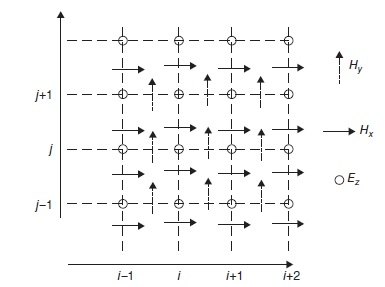
\includegraphics[width=10cm]{Interleaving_E_H.jpg}				
\caption{Campos Ez, Hx y Hy intercalados \cite{Houle2020}. }
\label{fig:EyH_intercalados}
\end{figure}
\noindent

Utilizaremos $\Delta x = \Delta y$, por lo que al haber elegido el tamaño de celda ($\Delta x \cdot \Delta y$), podemos calcular el salto temporal como:

\begin{equation}
\Delta t=\frac{\Delta x}{2 \cdot c_{0}}
\end{equation}

Donde $c_{0}$ es la velocidad de la luz en el vacío. Recordando que $\varepsilon_{0} \mu_{0}=1/(c_{0})^2$ y teniendo en cuenta la normalización utilazada:

\begin{equation}
    \frac{\Delta t}{\sqrt{\varepsilon_{0} \mu_{0}} \Delta x}=\frac{\Delta x}{2 \cdot c_{0}}\cdot 
     \frac{1}{\sqrt{\varepsilon_{0} \mu_{0}} \Delta x}=\frac{1}{2}
\end{equation}

Lo que nos permite, junto a las expresiones discretizadas en tiempo y espacio de las ecuaciones de Maxwell y la normalización empleada, generar un algoritmo de forma sencilla para calcular los campos:

\begin{align} \label{eq:actualizacion-campos}
	dz[i,j] &=dz[i,j] + 0.5*(hy[i,j]-hy[i-1,j]-hx[i,j]+hx[i,j-1]) \nonumber \\
    ez[i,j] &=gaz[i,j]*dz[i,j]  \nonumber \\
    hx[i,j] &=hx[i,j]+0.5*(ez[i,j]-ez[i,j+1]) \nonumber \\
    hy[i,j] &=hy[i,j]+0.5*(ez[i+1,j]-ez[i,j]) 
\end{align}

El valor $gaz[i,j]$ depende de las características del medio, por lo que si suponemos vacío su valor es 1. De este modo las ecuaciones \eqref{eq:actualizacion-campos} corresponden a los vectores necesarios para determinar los campos en $\mathbb R^{2}$, donde solo es necesario conocer el valor de la fuente que genera la radiación, ya sea cualquier tipo de fuente, sinusoidal o un pulso entre otros. 

En general, para conocer el valor del campo en todo el espacio es necesario calcular  su componente punto a punto pero utilizando la paralelización de la GPU podemos calcularlos todos los valores de los vectores a la vez.

\subsection{GPU} \label{subsection:GPU}

A lo largo de los años, debido a la necesidad de procesar gráficos de alta definición al instante, las tarjetas gráficas se han convertido en sistemas multinúcleo con la capacidad de multiproceso paralelizado. Las unidades de procesamiento de gráficos (GPUs) proporcionan más rendimiento y ancho de banda de memoria que las CPUs al mismo precio. Muchas aplicaciones aprovechan esta ventaja para ejercutarse más rapido en GPU que en CPU. La diferencia de potencia de las GPUs y las CPUs se basa en el propósito para el que fueron diseñadas las mismas. Las CPUs se crearon para que, con los pocos núcleos con que se construyen, ejecuten cálculos de forma secuencial en el menor tiempo posible. No obstante, las GPUs se crearon con miles de núcleos para que trabajen todos a la vez, realizando todos los cálculos paralelamente en vez de usar una metodología secuencial.

En la figura \ref{fig:arquitectura-cpu-gpu} se muestra la diferencia de estructura entre CPU y GPU, variando la cantidad de núcleos de la misma según el modelo de dispositivos utilizados. En general, dada la necesidad de ejecutar procesos tanto secuenciales como paralelos los sistemas están diseñados para poder mezclar los atributos de las CPUs y las GPUs maximizando así el rendimiento de los algoritmos \cite{web}.

\begin{figure}[h]
\centering
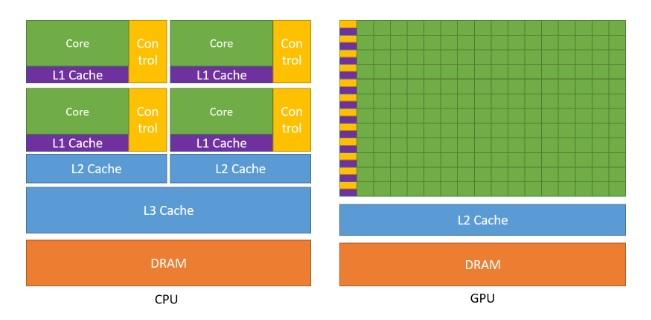
\includegraphics[width=15cm]{Nvidia-CPU-GPU.jpg}				
\caption{Diferencia de arquitectura entre CPU (izquierda) y GPU (derecha) \cite{web}. }
\label{fig:arquitectura-cpu-gpu}
\end{figure}
\noindent

Para generar soluciones que utilicen la paralerización de las tarjetas gráfics Nvidia ha desarrollado CUDA, un lenguaje de programación basado en C, el cual comparte sintaxis en muchos aspectos con este último lenguaje. En CUDA distinguimos dos tipos de procesos, los llevados a cabo en la CPU o 'host' y los ejecutados desde la GPU o 'device', teniendo acceso ambos dispositivos a dos tipos de memoria, global y constante. En la figura \ref{fig:arquitectura-cpu-gpu} se muestra al estructura del device y cómo ambos comparten memoria. Para identificar el lugar de ejecución de cada función cuda ha nombrado como \_\_host\_\_ a las aplicaciones ejecutadas en CPU y \_\_global\_\_ a las ejecutadas en GPU.

Cada tarjeta gráfica tiene un número determinado de threads o hilos, los cuales pueden realizar un cálculo concreto simultaneamente cuando son llamados por una función global (desde el device). Para realizar esta llamada CUDA divide los núcleos en bloques y mallas como se puede ver en la figura \ref{fig:componentes gpu}, donde se muestra una malla de dos bloques y dos hilos en cada bloque, siendo 4 los hilos totales. Destacar que en general el número de hilos tiene que coincidir necesariamente con el número de núcleos ya que, como ocurre en las CPUs, puede haber varios hilos en un mismo núcleo. Esto significa que dentro de un mísmo núcleo pueden realizarse tantos cálculos simultáneos como hilos tenga dicho procesador, no obstante la diferencia de hilos entre un procesador y una gráfica es de varios órdenes de magnitud, pudiendo ser 6 en una CPU y miles en una GPU.

\begin{figure}[h]
\centering
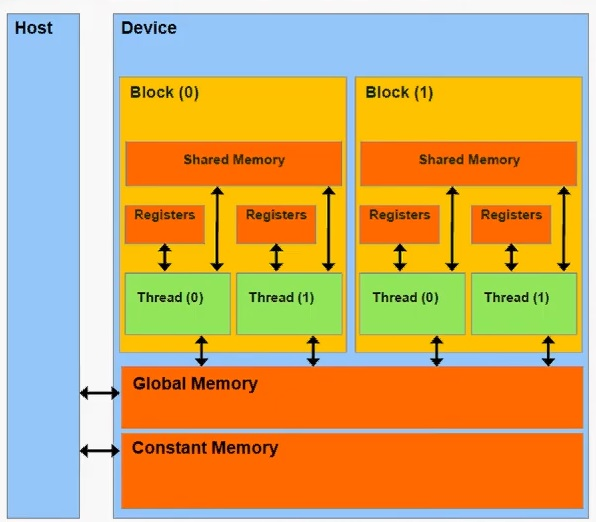
\includegraphics[width=10 cm]{Nvidia-Device_Structure.jpg}				
\caption{Estructura del Host (\cite{web}). }
\label{fig:componentes gpu}
\end{figure}
\noindent

Al implementar una solución, desde el host se selecciona el número de hilos a utilizar teniendo en cuenta las limitaciones de hilos por bloques y bloques por mallas de la tarjeta gráfica que se esté utilizando y desde la función global (en el device) se determinan las operaciones a realizar por cada hilo. Es decir, antes de ejecutar la función \_\_globla\_\_ se debe conocer el número de hilos y bloques a utilizar por la GPU, pudiendo lanzar un número determinado de estos en las tres dimensiones del espacio (x,y,z).

Dadas las variables a utilizar, hilos, bloques y mallas, es necesario identificar el hilo que se quiere utilizar para ejecutar el cálculo. Conceptualmente podemos ver una malla como una matriz, dividida por bloques e hilos dentro de estos bloques como se muestra en la figura \ref{fig:hilos, bloques y mallas en gpu}. En ella podemos ver una malla compuesta por 60 hilos, dividida por 4 bloques, dos en la dimensión x denotada por 'gridDim.x', dos en la dimensión y denotada por 'gridDim.y', estando cada bloque compuesto de 15 hilos.

\begin{figure}[h]
\centering
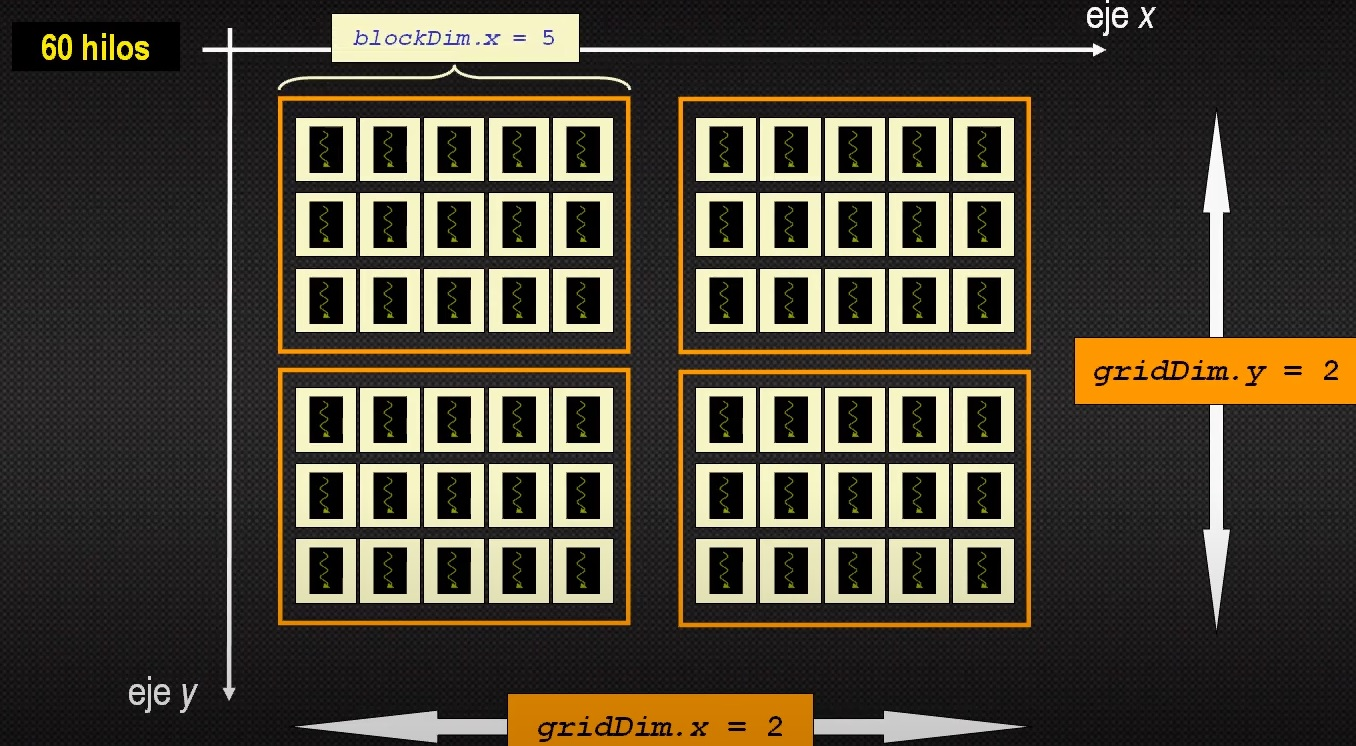
\includegraphics[width=10 cm]{Nvidia_Topologia_virtual.jpg}				
\caption{Topología dentro de hilos, bloques y mallas (Documentación de Nvidia [3]) }
\label{fig:topologia-hilos}
\end{figure}
\noindent

No obstante, la división que hace CUDA de los hilos es lineal como se muestra en la figura \ref{fig:topologia-hilos}. En ella podemos ver separados por franjas claras y oscuras el paso de un bloque a otro. De modo que, para poder identificar un hilo podemos concebir la malla como una matriz donde las filas determinan el bloque y las columnas los hilos. Así, se distingue unívocamente cada hilo multiplicando las columnas totales por el número del bloque donde está el hilo y sumandole la posición que ocupa en el.

\begin{figure}[h]
\centering
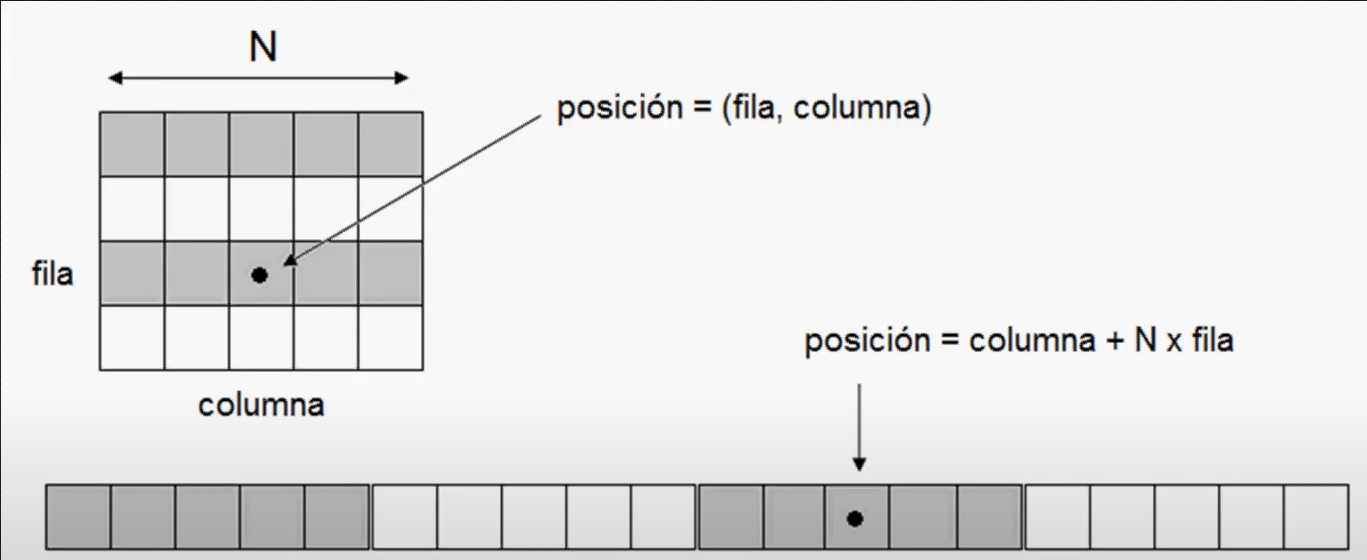
\includegraphics[width=10 cm]{Nvidia_Posicion_hilo.jpg}				
\caption{Identificación de hilo dentro de una malla.}
\label{fig:localizacion de hilos}
\end{figure}
\noindent

En nuesto caso, debido a las necesidades del problema necesitamos identificar los hilos de una malla lanzada con hilos y bloques en dos dimensiones. Por lo que necesitamos identificar qué son las filas y las columnas en nuestra función \_\_globla\_\_. Esta identificación la conseguimos usando las palabras reservadas que nos proporciona CUDA:

\begin{verbatim}
     int fil = blockIdx.y * blockDim.y + threadIdx.y;
     int col = blockIdx.x * blockDim.x + threadIdx.x;
\end{verbatim}

Es necesario resaltar la necesidad de seleccionar la cantidad de hilos y bloques acorde a la capacidad de la gráfica y las necesidades del problema. En específico, para la resolución de las ecuaciones de Maxwell en dos dimensiones para un mallado de un millón de puntos, dividido en 1000 posiciones en la dimensión x y 1000 posiciones en la dimensión y, con la gráfica utilizada en este TFG (la cual perrmite 1024 hilos por bloque), es necesario utilizar un mínimo de 977 bloques de 1024 hilos cada uno.


Finalmente, para medir el tiempo de cálculo en el device CUDA nos proporciona la función 'cudaEvent', con la cual se establecen dos marcas de tiempo en el algoritmo y se calcula el tiempo como la resta de estas mismas, siendo la diferencia el tiempo transcurrido en el device al realizar las operaciones.
Para calcular el tiempo en el host se ha utilizado la función 'clock\_t' y de la misma forma se han creado dos marcas temporales y se ha calculado la diferencia. En ambos casos se han dividido los resultados entre las cuentas por segundo dentro del procesador y la tarjeta gráfica para obtener el tiempo en segundos.

\section{Implementación}

\url{https://github.com/juanjo1213/TFG-FDTD}

En el mismo están los algoritmos utilizados para la solución en 2D implementada tanto en la cpu y en la gpu. La implementación de la solución en el device está nombrada como 'fd2d\_simp.cu' y la ejecutada en el host como 'HOST\_FD2D\_SIMP.cu'.

\begin{verbatim}
	__host__ void check_CUDA_Error(const char* mensaje)
	{
		cudaError_t error;
		cudaDeviceSynchronize();
		error = cudaGetLastError();
		if (error != cudaSuccess)
		{
			printf("ERROR %d: %s (%s)\n", error, cudaGetErrorString(error), mensaje);
            printf("\npulsa INTRO para finalizar...");
            fflush(stdin);
        	char tecla = getchar();
			exit(-1);
		}
	}
\end{verbatim}

%\begin{figure}[h]
%\centering
%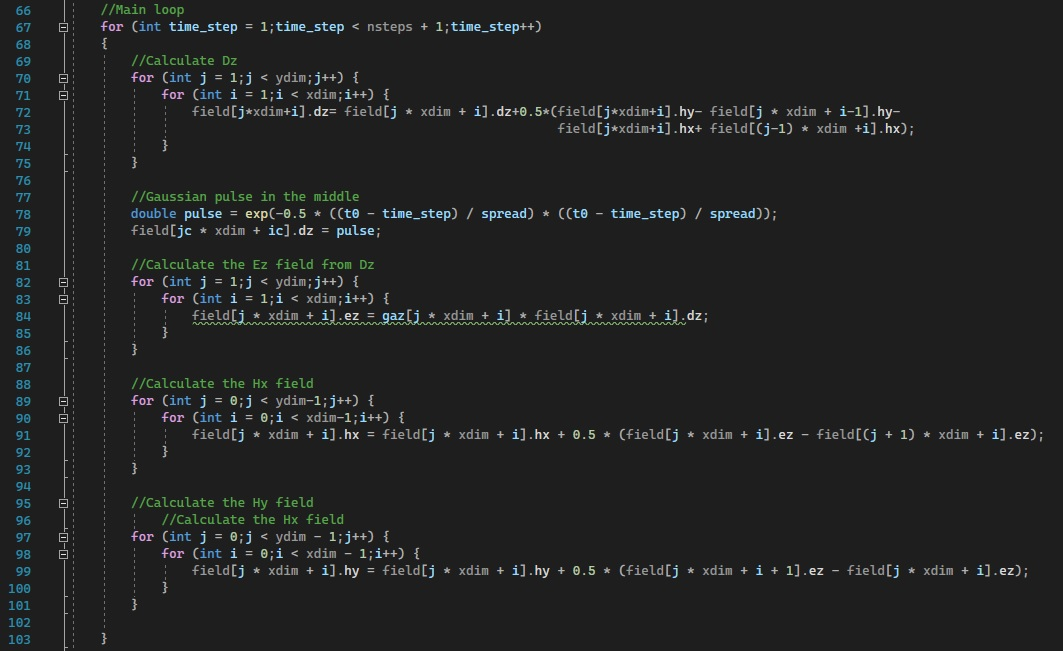
\includegraphics[width=15cm]{FD2D_Host_loop.jpg}				
%\caption{Implementación de las ecuaciones (2.21-2.24) para el cálculo de los campos en la CPU }
%\end{figure}
%\noindent


Para la ejecución de los algoritmos se ha utilizado un procesador i7-6700K procesador de 4 núcleos y 8 hilos con una frecuencia máxima de 4.2 GHz por núcleo y una tarjeta gráfica GTX 1070 con 8GB de memoria RAM y un total de 1920 núcleos CUDA. 

A continuación se muestra la función \_\_host\_\_ generada para el cálculo de las ecuaciones \ref{eq:actualizacion-campos}, esta es llamada desde el host y recibe como parámetro un 'struct' que contiene los vectores campo a calcular. En ella se ejecutan varios bucles para el cálculo secuencial de los campos punto a punto y para mayor similitud, se han almacenado las matrices como vectores de dimensión $dimx\cdot dimy$ y se ha determinado cada componente a calcular como se expuso en la sección \ref{subsection:GPU}. 


\begin{verbatim}
void FD2D(FDTDData* field, int xdim, int ydim, int nsteps)
{
 int ic = int(xdim / 2),
  jc = int(ydim / 2);

 //Medium conditions
 double* gaz;

 gaz = (double*)malloc(xdim * ydim * sizeof(double));

 for (int j = 0;j < ydim;j++) {
  for (int i = 0;i < xdim;i++) {
   gaz[j * xdim + i] = 1.0;
  }
 }


 double ddx = 0.01,         //cell size
     dt = ddx / 6e8,     //Time step size
     epsz = 8.854e-12;   //Dielectric profile



 //Pulse parameters
 double t0 = 20.0,
  spread = 6.0;

 //Main loop
 for (int time_step = 1;time_step < nsteps + 1;time_step++)
 {
  //Calculate Dz
  for (int j = 1;j < ydim;j++) {
   for (int i = 1;i < xdim;i++) {
    field[j*xdim+i].dz= field[j * xdim + i].dz+
                        0.5*(field[j*xdim+i].hy- field[j * xdim + i-1].hy-
                        field[j*xdim+i].hx+ field[(j-1) * xdim +i].hx);
   }
  }

  //Gaussian pulse in the middle
  double pulse = exp(-0.5 * 
           ((t0 - time_step) / spread) * ((t0 - time_step) / spread));
  field[jc * xdim + ic].dz = pulse;

  //Calculate the Ez field from Dz
  for (int j = 1;j < ydim;j++) {
   for (int i = 1;i < xdim;i++) {
    field[j * xdim + i].ez = gaz[j * xdim + i] * field[j * xdim + i].dz;
   }
  }

  //Calculate the Hx field
  for (int j = 0;j < ydim-1;j++) {
   for (int i = 0;i < xdim-1;i++) {
    field[j * xdim + i].hx = field[j * xdim + i].hx + 
            0.5 * (field[j * xdim + i].ez - field[(j + 1) * xdim + i].ez);
   }
  }

  //Calculate the Hy field
   //Calculate the Hx field
  for (int j = 0;j < ydim - 1;j++) {
   for (int i = 0;i < xdim - 1;i++) {
    field[j * xdim + i].hy = field[j * xdim + i].hy + 
          0.5 * (field[j * xdim + i + 1].ez - field[j * xdim + i].ez);
   }
  }

 }




}
\end{verbatim}

En el siguiente algoritmo se muestra la función \_\_global\_\_ generada para realizar los cálculos de forma paralela. En ella podemos ver como se determinan las filas y las columnas utilizadas para determinar los hilos a utilizar como se explicó en la sección \ref{subsection:GPU}. La función, al igual que la función anteior, recibe como parámetro un struct que contiene los vectores a clacular, las dimensiones $x$ e $y$ del problema y el paso temporal que se está ejecutando. Al existir la posibilidad de reservar más bloques e hilos de los necesarios para realizar los cálculos, se usa el condicional 'if' para especificar el número de hilos a utilizar.

\begin{verbatim}
    __global__ void FD2D(FDTDData* field, int xdim, int ydim, int ts)
{
 int fil = blockIdx.y * blockDim.y + threadIdx.y;
 int col = blockIdx.x * blockDim.x + threadIdx.x;


 int ic = int(xdim / 2),
  jc = int(ydim / 2);

 double ddx = 0.01,
  dt = ddx / 6e8,
  epsz = 8.854e-12;

 //pulse parameters
 double t0 = 20.0,
  spread = 6.0;

 //Calculate Dz
 if (0 < fil && fil < ydim && 0 < col && col < xdim) {
  field[fil * xdim + col].dz += 0.5 * 
      (field[fil * xdim + col].hy - field[fil * xdim + col - 1].hy -
   field[fil * xdim + col].hx + field[(fil - 1) * xdim + col].hx);
 }
 __syncthreads();

 //Gaussian pulse in the middle
 double pulse = exp(-0.5 * ((t0 - ts) / spread) * ((t0 - ts) / spread));
 field[jc * xdim + ic].dz = pulse;
 __syncthreads();

 //Calculate the Ez field from Dz
 if (0 < fil && fil < ydim && 0 < col && col < xdim) {
  field[fil * xdim + col].ez = field[fil * xdim + col].gaz * 
                               field[fil * xdim + col].dz;
 }
 __syncthreads();

 //Calculate the Hx field
 if (fil < ydim - 1 && col < xdim - 1) {
  field[fil * xdim + col].hx += 0.5 * (field[fil * xdim + col].ez - 
                                     field[(fil + 1) * xdim + col].ez);
 }
 __syncthreads();

 //Calculate the Hy field
 if (fil < ydim - 1 && col < xdim - 1) {
  field[fil * xdim + col].hy += 0.5 * 
        (field[fil * xdim + col + 1].ez - field[fil * xdim + col].ez);
 }

}
\end{verbatim}

En ambas funciones se emplea un bucle ya sea dentro o fuera de la función para especificar el número de pasos temporales a realizar, además de utilizar como fuente de los campos un pulso gaussiano, denotado en ambas funciones como 'pulse' y generado en el centro del espacio.





\section{Resultados}

Al resolver las ecuaciones \ref{eq:actualizacion-campos}, como cabe esperar, obtenemos una onda electromagnética propagandose por el espacio, la cual es generada por un pulso gaussiano como fuente. La figura \ref{fig:solucion} muestra la propagación del campo eléctrico (Ez) en un espacio de 3600 puntos y 20, 30, 40, 50 pasos temporales. Como podemos ver, la onda generada en el centro se propaga en las direcciones $x$ e $y$.  

\begin{figure}[h]
\centering
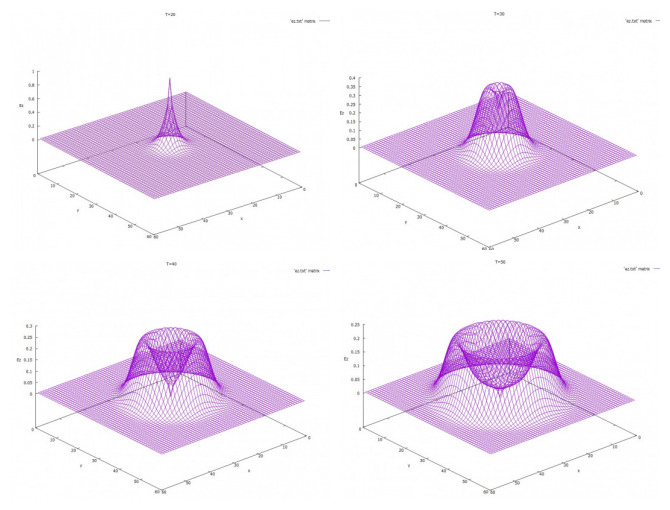
\includegraphics[width=15 cm]{Solution.JPG}				
\caption{Propagación del campo eléctrico en $\mathbb R^{2}$ en un espacio de 3600 puntos en 20 (Superior-Izquierda), 30 (Superior-Derecha), 40 (Inferior-izquierda) y 50 (Inferior-Derecha) pasos temporales.}
\label{fig:solucion}
\end{figure}
\noindent

Para determinar la ganancia en tíempo de cálculo al implementar este algoritmo en CUDA se han realizado dos experimenteos, donde se prueba la dependencia de este con el número de pasos temporales y la densidad de puntos.

\subsection{Dependencia del tiempo de cálculo con el número de pasos temporales}

Para determinar la dependencia del tiempo de cálculo con el número de pasos temporales se han llevado a cabo diez ejecuciones, cinco utilizando el host y cinco utilizando el device. En las diez se ha utilizado una densidad constante de puntos de 25 millones y se han variado los pasos temporales desde 10 hasta 10 000. En las tablas \ref{tab:npasosCPU} y \ref{tab:npasosGPU} se enumeran los datos obtenidos en las ejecuciones realizas.

\begin{table}[h]
    \centering
    \begin{tabular}{|c|c|c|c|}
    \hline
    \multicolumn{4}{ |c| }{CPU} \\ \hline
         Densidad de puntos & Pasos Temporales &  $t_{CPU}$ ($\pm 1$ segundos) & Minutos ($\pm 0.01$)  \\ \hline \hline
        25 000 000 & 10 & 1 & 0.01 \\ \hline
         25 000 000 & 100 & 19 & 0.32 \\ \hline
         25 000 000 & 1000 & 204 & 3.40 \\ \hline
         25 000 000 & 5000 & 1105 & 18.42 \\ \hline
         25 000 000 & 10000 & 2199 & 37.05 \\ \hline
    \end{tabular}
    \caption{Dependencia del tiempo de cálculo con los pasos temporales en CPU}
    \label{tab:npasosCPU}
\end{table}



\begin{table}[h]
    \centering
    \begin{tabular}{|c|c|c|c|}
    \hline
    \multicolumn{4}{ |c| }{GPU} \\ \hline
         Densidad de puntos & Pasos Temporales &  $t_{GPU}$ ($\pm 1$ segundos) & Minutos ($\pm 0.01$)  \\ \hline \hline
         25 000 000 & 10 & 0 & 0.00 \\ \hline
         25 000 000 & 100 & 0 & 0.00 \\ \hline
         25 000 000 & 1000 & 16 & 0.27 \\ \hline
         25 000 000 & 5000 & 87 & 1.45 \\ \hline
         25 000 000 & 10000 & 173 & 3.28 \\ \hline
    \end{tabular}
    \caption{Dependencia del tiempo de cálculo con los pasos temporales en GPU}
    \label{tab:npasosGPU}
\end{table}

Como podemos ver en ellas

\begin{figure}[h]
\centering
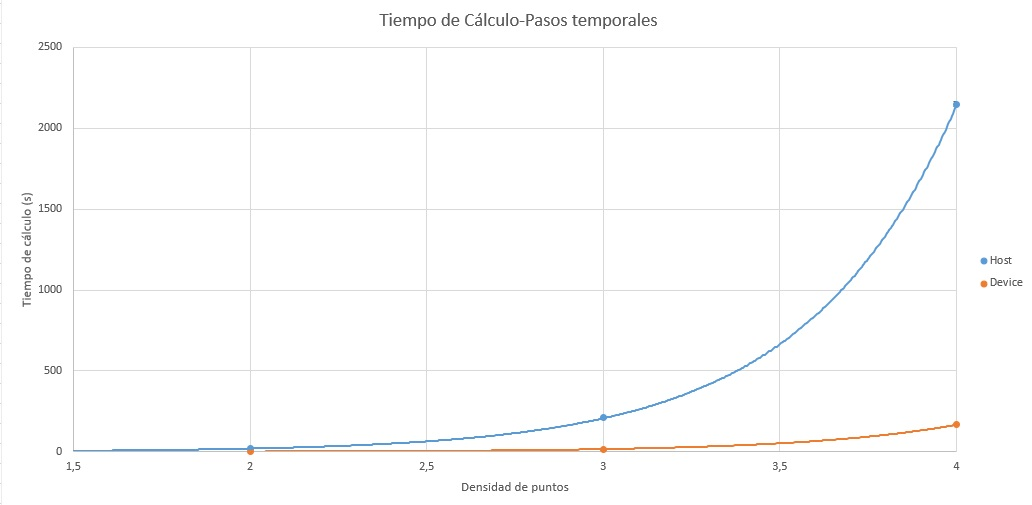
\includegraphics[width=15 cm]{T-Pasos_temporales.jpg}				
\caption{Relación entre el tiempo de cálculo y el número de pasos temporales para una densidad de puntos de 25 millones. La línea naranja representa el tiempo de ejecución en el device y la azul el tiempo de ejecución en el host}
\label{fig:t-pasos_temporales}
\end{figure}
\noindent




\begin{table}[h]
    \centering
    \begin{tabular}{|c|c|}
    \hline
         Pasos Temporales &  $t_{CPU}$ - $t_{GPU}$ ($\pm 1.4$ segundos)   \\ \hline \hline
         10 & 1  \\ \hline
          100 & 19  \\ \hline
          1000 & 188  \\ \hline
          5000 & 1018  \\ \hline
          10000 & 2626  \\ \hline
    \end{tabular}
    \caption{t}
    \label{tab:1}
\end{table}

\begin{figure}[h]
\centering
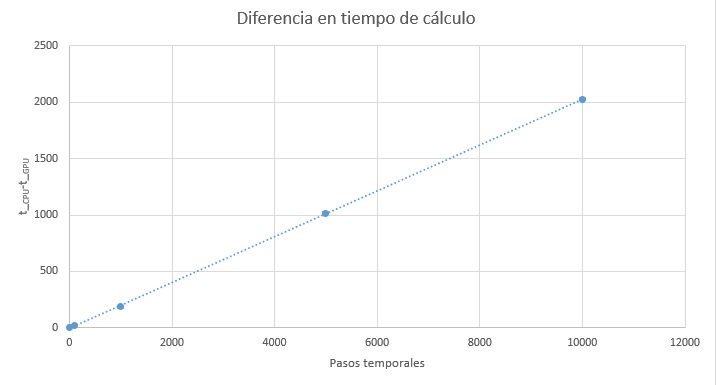
\includegraphics[width=15 cm]{DiferenciaEntiempoDeCalculo.jpg}				
\caption{Diferencia en tiempo de cálculo}
\label{fig:diferencia_en_tiempo_de_calculo}
\end{figure}
\noindent


\subsection{Variación del tiempo de cálculo al variar la densidad de puntos}

En la determinación de la dependencia del tiempo de cálculo con la densidad de puntos también se han llevado a cabo diez ejecuciones, cinco en el host y cinco en el device, donde se ha determinado el tiempo de cálculo para un número de 1000 pasos temporales y una densidad de puntos desde 10 millones hasta 25 millones. En las tablas \ref{tab:densidad_de_puntos_CPU} y \ref{tab:npasosGPU} podemos ver los datos obtenidos tras las diez eejcuciones.

\begin{table}[h]
    \centering
    \begin{tabular}{|c|c|c|c|}
    \hline
    \multicolumn{4}{ |c| }{CPU} \\ \hline
         Densidad de puntos & Pasos Temporales &  $t_{CPU}$ ($\pm 1$ segundos) & Minutos ($\pm 0.01$)  \\ \hline \hline
        10 000 00 & 1000 & 7 & 0.11 \\ \hline
        4 000 000 & 1000 & 32 & 0.53 \\ \hline  
        9 000 000 & 1000 & 71 & 1.18 \\ \hline
        16 000 000 & 1000 & 126 & 2.10 \\ \hline
        25 000 000 & 1000 & 204 & 3.17 \\ \hline
    \end{tabular}
    \caption{Dependencia del tiempo de cálculo con la densidad de puntos utilizados en CPU}
    \label{tab:densidad_de_puntos_CPU}
\end{table}



\begin{table}[h]
    \centering
    \begin{tabular}{|c|c|c|c|}
    \hline
    \multicolumn{4}{ |c| }{CPU} \\ \hline
         Densidad de puntos & Pasos Temporales &  $t_{GPU}$ ($\pm 1$ segundos) & Minutos ($\pm 0.01$)  \\ \hline \hline
        10 000 00 & 1000 & 0 & 0.0 \\ \hline
        4 000 000 & 1000 & 2 & 0.03 \\ \hline  
        9 000 000 & 1000 & 6 & 0.10 \\ \hline
        16 000 000 & 1000 & 10 & 0.17 \\ \hline
        25 000 000  & 1000 & 16 & 0.27 \\ \hline
    \end{tabular}
    \caption{Dependencia del tiempo de cálculo con la densidad de puntos utilizados en GPU}
    \label{tab:densidad_de_puntos_GPU}
\end{table}

Como podemos ver en las tablas el tiempo de ejecución crece significativamente al aumentar la densidad de puntos utilizada en la implementación del host. No obstante, al utilizar la paralelización ofrecida por CUDA el aumento en tiempo de cómputo es menos abrupto.

Esta diferencia podemos verla de forma más clara en la figura \ref{fig:t-densidad_de_puntos}, en ella vemos el aumento en tiempo de ejecución del algoritmo ejecutado en el host en azul y el aumento en tiempo de ejecución del algoritmo implementado en el device en naranja.

\begin{figure}[h]
\centering
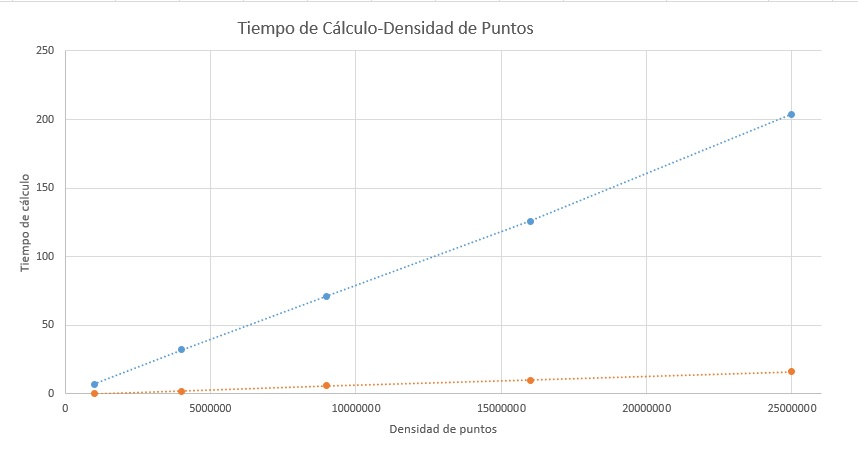
\includegraphics[width=15 cm]{T-Densidad_de_Puntos.jpg}				
\caption{Relación entre el tiempo de cálculo y la densidad de puntos para 1000 pasos temporales. La línea naranja representa el tiempo de ejecución en el device y la azul el tiempo de ejecución en el host}
\label{fig:t-densidad_de_puntos}
\end{figure}
\noindent

sadfa








\section{Conclusiones}



% Referencias %%%%%%%%%%%%%%%%%%%%%%%%%%%%%%%%%%%%%%%%%%%%%%%%%%%%%%%%%%%%%%%%%
\newpage

\addcontentsline{toc}{section}{Referencias} % Elige según idioma
%\addcontentsline{toc}{section}{References} % Elige según idioma

\begin{thebibliography}{100}

\bibitem{Houle2020}
  Jennifer E~Houle and Dennis M~Sullivan, \\
  {\em Electromagnetic simulation using the FDTD method with Python}, \\
  IEEE PRESS WILEY, 2020.
  
\bibitem{Taflove2005}
Allen Taflove and Susan C~Hagness, \\
{\em Computational electrodynamics. The Finite-Difference Time-Domain Method}, \\
ARTECH HOUSE, 2005.

\bibitem{web}
 Nvidia documentation, \\
 \href{https://docs.nvidia.com/cuda/cuda-c-programming-guide/index.html}{https://docs.nvidia.com/cuda/cuda-c-programming-guide/index.html}






%\ \bibitem{PYTHIA}
%\   T.~Sjostrand, S.~Mrenna and P.~Z.~Skands, \\
%\   {\em PYTHIA 6.4 Physics and Manual}, \\
%\   JHEP {\bf 0605} (2006) 026  [hep-ph/0603175].
%\   
%\ \bibitem{conferencia}
%\   F.~Wilczek, \\
%\   {\em A long view of particle physics}, \\
%\   Proceedings of the 25th Solvay Conference on Physics, p. 210-249, \\  
%\   Brussels, Belgium, October 19-25, 2011.
%\ 
%\ \bibitem{charla}
%\   D.~Gross, \\
%\   {\em Quantum Field Theory: Past, Present and Future}, \\
%\   Talk at the Conference in Honour of the 90th Birthday of Freeman Dyson, \\
%\   Institute of Advanced Studies, Singapore, August 26-29, 2013.
%\ 
%\ \bibitem{libro}
%\   M.~E. Peskin and D.~V. Schroeder, \\
%\   {\em An Introduction to Quantum Field Theory}, \\
%\   Addison-Wesley, 1995.
%\   
%\ \bibitem{tesis}
%\   M.~R.~Chala, \\
%\   {\em Collider Signatures of a Non-Standard Higgs Sector}, \\
%\   PhD Thesis, Universidad de Granada, 2014.
%\ 
%\ \bibitem{web}
%\  Particle Physics News and Resources, \\
%\  \href{http://www.interactions.org/}{http://www.interactions.org/}
 
\end{thebibliography}

\end{document}
